\section{Greedy Index Construction}
\label{preprocessing}

This section describes the greedy index construction algorithm. For a vertex, all shortest paths from a landmark can be indexed as its label. We focus on the problem of deciding which shortest path to be indexed, so that better online query accuracy for average cases can be achieved. 

\begin{figure*}[ht]
		\vspace{-1cm}
    \centering
    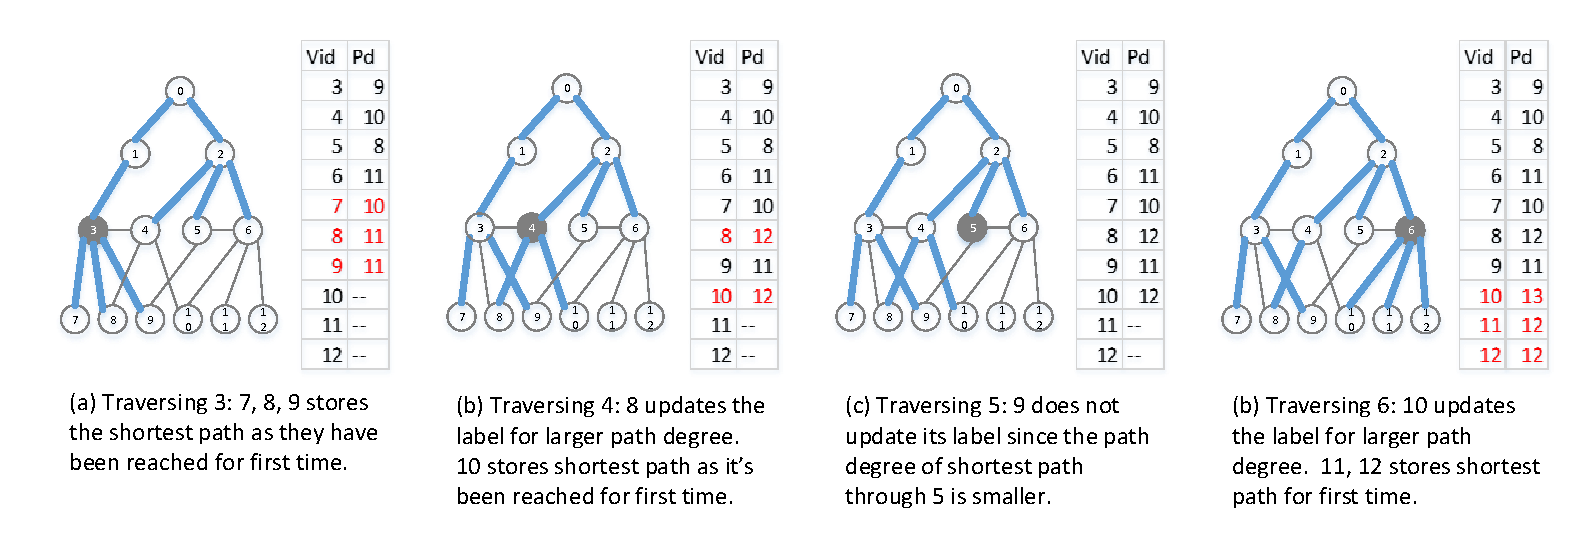
\includegraphics[width=\linewidth]{./figures/new_illustrate/bfs_illustrate.pdf}
		\vspace{-1cm}
    \caption{Heuristic index construction pick shortest path with highest path degree during breadth first search}
    \label{fig:bfs_illustrate}
		\vspace{-5mm}
\end{figure*}

As the core of decentralized search is to iteratively find neighbor vertices that have shortest LCA distances to the target. From the point of view of a vertex $u$, if the indexed shortest path intersects with many indexed shortest paths of other vertices, the possibility that other vertices have a small LCA distance to $u$ is going to be higher. With this intuition, we design our heuristic greedy index construction algorithm to store the shortest path with the highest ``centrality'', i.e., a path that intersects with most other shortest paths. To represent the ``centrality'' of a shortest path, we use the sum of vertex degrees along the path. %Although betweenness centrality fits our needs very well, its computation cost is too high~\cite{Riondato:2014:FAB:2556195.2556224}. Therefore, we use degrees as an alternative and refer to the sum of degrees of vertices along a path as path degree, denoted by $Pd$.

%Based on the path degree concept, our index construction procedure can be easily modified to index the shortest path with the highest path degree. 
As path degrees of shortest paths follow optimal substructures, 
%i.e., if a shortest path $(u, .., w, ..., v)$ has the highest path degree among all the shortest paths from $u$ to $v$, then the path degree of $(u, ..., w)$ is also the highest among all the shortest paths from $u$ to $w$.
to index the shortest path with the highest path degree, during BFS, suppose the search is visiting vertex $u$ and reach its neighbor $v$ with non empty $L(v)$, we perform a label update if $|L(v)| > |L(u)|$ and $Pd(u) + \rho(v) > Pd(v)$, where $\rho(v)$ denote the degree of vertex $v$. The detailed algorithm of greedy index construction is depicted in Algorithm~\ref{alg:index_construct}. 

Fig.~\ref{fig:bfs_illustrate} shows an example of how to greedily select the shortest path with the highest path degree during BFS. When traversing vertex $4$, even though vertex $8$ has already been indexed with a shortest path $(0, 1, 3, 8)$ into its label, due to that $(0, 2, 4, 8)$ has a higher path degree, the label of vertex $8$ is updated. The same happens to vertex $10$ while traversing vertex $6$. 

\begin{algorithm}[h]
    \caption{Greedy index construction on landmark $l$}
		\label{alg:index_construct}
    \begin{algorithmic}
				\Function{Index construction}{$l$}
						\State For each $v$ in $G$: $L(v) \gets \emptyset$
						\State For each $v$ in $G$: $Pd(v) \gets 0$
						\State $Q \gets \emptyset$
						\State $L(l) = l$
						\State $Pd(l) = \rho(l)$ \
						\Comment {$\rho$ denotes degree}
						\State $Q.push(l)$
						\While{$Q \neq \emptyset$}
								\State $u = Q.pop()$
								\For{each $v_i$ adjecent to $u$}
										\If{$L(v_i) = \emptyset$}
												\State $L(v_i) = L(u)$
												\State append $v_i$ to $L(v_i)$
												\State $Pd(v_i) = Pd(u) + \rho(v_i)$
												\State $Q.push(v_i)$
										\ElsIf{$|L(v_i)| > |L(u)|$ {\bf and} $Pd(v_i) < Pd(u) + \rho(v_i)$}
												\State $L(v_i) = L(u)$
												\State append $v_i$ to $L(v_i)$
												\State $Pd(v_i) = Pd(u) + \rho(v_i)$
										\EndIf
								\EndFor
						\EndWhile
						\State \Return $L$
        \EndFunction
    \end{algorithmic}
\end{algorithm}

Note that if the landmark set is relatively large, then following the highest path degree heuristic may lead to redundant labels, i.e., similar indexed shortest path trees for multiple landmarks, which can compromise the accuracy of online searches. A simple way to solve this problem is to prioritize shortest paths which overlap less with shortest paths that have already been indexed.